\phantomsection
\label{sec:appendix}\npsectionstar{Appendix: figures}
\vfill
\begin{figure}[H]
    \centering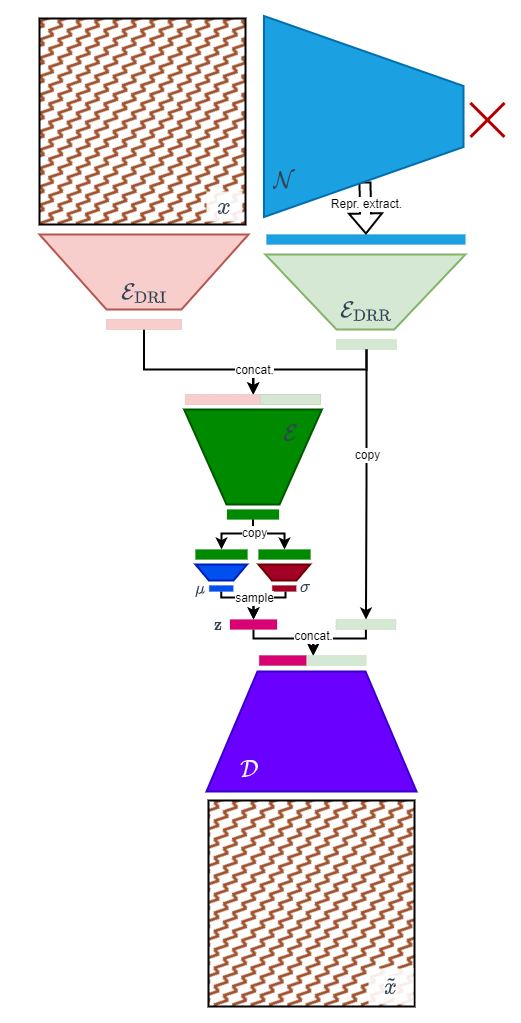
\includegraphics[ width=0.8\textwidth,height=0.8\textheight,keepaspectratio]{img/traindiag.png}
    \caption{Essentialised \texttt{CARSO} architecture at training time. Square elements denote \textit{inputs} or their reconstruction (the same colours and graphical pattern are used regardless of implied similarity). The size of the elements is not necessarily in scale (an estimation based on typical scenarios has been made).}
\end{figure}
\vfill
\newpage

\null\vfill
\begin{figure}[H]
    \centering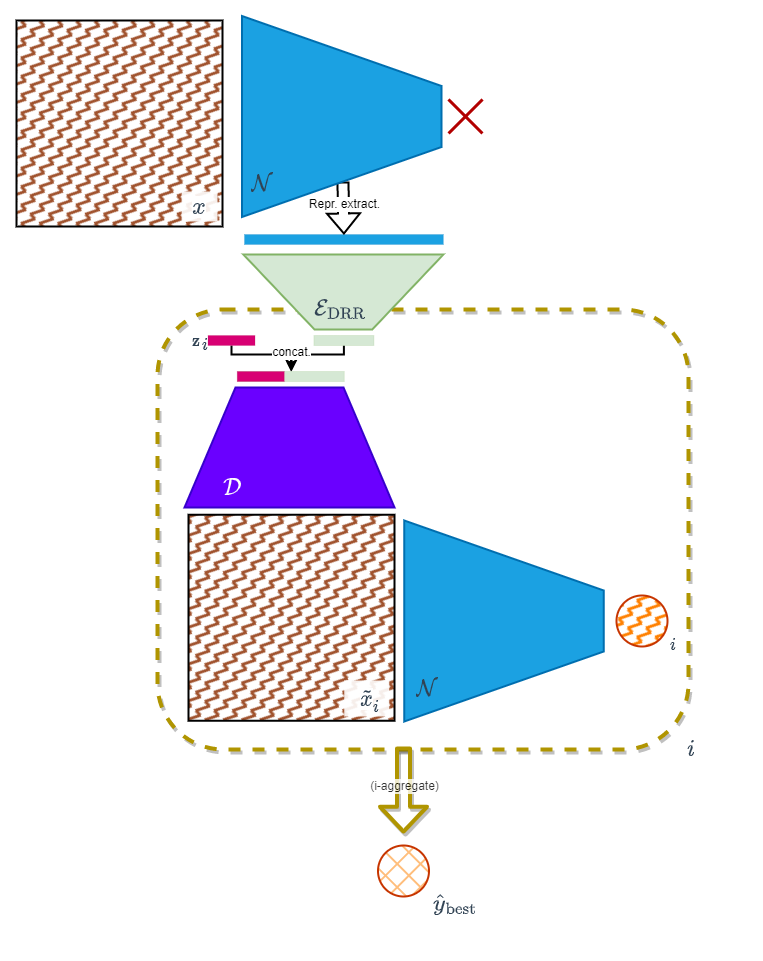
\includegraphics[ width=0.8\textwidth,height=0.8\textheight,keepaspectratio]{img/inferdiag.png}
    \caption{Essentialised \texttt{CARSO} architecture at inference time. Square elements denote \textit{inputs} or their reconstruction (the same colours and graphical pattern are used regardless of implied similarity). Round elements denote the output class of the classifier taken into consideration. The region bordered by the dashed line constitutes the input-reconstruction \textit{sampler} (followed by the classifier $\mathcal{N}$), whose use can be arbitrarily repeated, for fixed input $\vec{x}$. The size of the elements is not necessarily in scale (an estimation based on typical scenarios has been made).}
\end{figure}
\vfill